\documentclass[12pt]{article}
\usepackage{amsmath,amssymb,amsthm}
\usepackage{graphicx,mathabx}
\usepackage{xcolor}
\usepackage{tikz}
\usepackage{placeins}
\usepackage{lipsum}
\usepackage[shortlabels]{enumitem}
\usepackage{placeins}
\usepackage[makeroom]{cancel}
\usepackage{mathrsfs}
\newcommand\tab[1][1cm]{\hspace*{#1}}
\def\blankpage{%
      \clearpage%
      \thispagestyle{empty}%
      \addtocounter{page}{-1}%pdf
      \null%
      \clearpage}
\begin{document}
\title{TCSS 343 - Week 7}
\author{Jake McKenzie}
\maketitle
\noindent\centerline{\textbf{Greedy Algorithms}}\\\\\\\\\\\\\\\\
\begin{center}
    ``Finding a needle in a haystack is actually quite easy. It's finding a very specific piece of hay in a haystack that happens to be hard." \\$\dots$\\ Avi Wigderson
\end{center}
\begin{center}
    In his first computer science class Ryan Williams was not afraid to tell his instructor that he thought it was too easy. Eventually, his frustrated teacher pulled a heavy white book off of a shelf, dumped it dramatically on Williams' desk, and told him to look up the problem described in the final chapter. ``If you can solve that," he said, ``then you can complain." That book was CLRS' Introduction to Algorithms and the problem was P vs. NP.
\end{center}
\begin{center}
    ``It is not enough to be in the right place at the right time. You should also have an open mind at the right time." \\$\dots$\\ Paul Erd\H{o}s
\end{center}
\newpage
\noindent 0. With this problem I want to present a 
problem to you and ask you why the greedy algorithm fails.\\\\
Imagine we have a wizard that knows a few spells. 
Each spell has 3 attributes: Damage, cooldown time, and a cast time. \\\\
\textbf{Cooldown time:} the amount of time (t) it takes 
before being able to cast that spell again. 
A spell goes on ``cooldown" the moment it begins casting.\\\\
\textbf{Cast time:} the amount of time (t) it takes 
to use a spell. While the wizard is casting 
something another spell cannot be cast and 
it cannot be canceled. \\\\
\textit{The question is:} \textbf{How would you maximize damage 
given different sets of spells?} \\\\
It is easy to calculate the highest damage per cast 
time. But what about in situations where it is better 
to wait then to get ``stuck" casting a low damage 
spell when a much higher one is available...for example consider
the two sets of spells:\\\\\\
Chill Touch: $100$ damage at a rate of $1$ second per cast with a $10$ second cooldown. \\\\
Mage Hand. $10$ damage at a rate of $4$ second per cast with a $0$ second cooldown.\\\\
Optimal spell ordering $\Sigma =\{$Chill Touch, Mage Hand, Wait, Repeat$\}$\\\\
0. Given an arbitary amount of time $t$ what is the maximum amount of spells
we can cast $S$?
\newpage
\noindent Now imagine that there is one spell, henceforth called the Eldritch Blast, 
which does a very, very large amount of damage, has $0$ casting time, and has 
some positive cooldown $n$. If all the other spells do much less damage than the 
Eldritch Blast, it will clearly be optimal to cast the Eldritch Blast every n seconds and 
then optimize the cooldown time with the weaker spells.\\\\
1. Why does the greedy algorithm work in this case?\\\\\\\\\\\\\\\\\\\\
Now, assume all the other spells also have cooldown $n$. 
If one optimizes a given n-second downtime with these spells, 
then the same spell-sequence will also be possible in the next 
$n$-second downtime, and so we can assume the solution is $n$-periodic.\\\\
2. Why does the greedy algorithm work in this case?\\\\\\\\\\\\\\\\\\\\
3. Would you say this problem is NP-Complete? NP-Complete problems have the 
highest complexity of any problem in NP, which are the class of problems which can
be quickly checked to be true.
\newpage
\noindent For this problem and many problems, we can abstract out the details like we just did
and reduce the problem to it's key constituent parts. When you employ this
design technique you'll begin to notice that many problems you have reduce to problems
to classes of problems. This is the most powerful design technique I know of when it 
comes to algorithms.\\\\
4. Of the problems you've covered in class, which does this problem degenerate too? Describe for 
which cases this problems degrenates to that problem you've already covered.\\\\\\\\\\\\\\\\\\\\\\\\\\\\\\\\
5. Can you produce an informal algorithm that attempts to solve this problem?
\newpage
\centerline{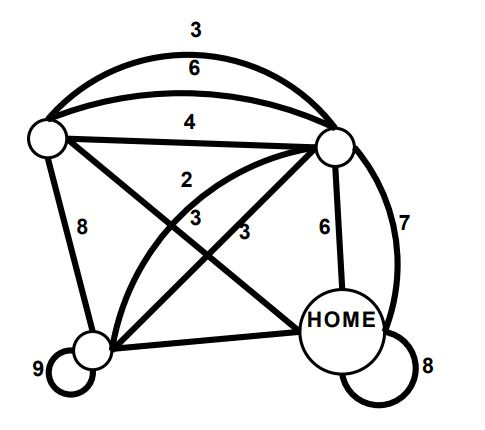
\includegraphics[scale = .45]{jogger.jpg}}
\noindent 6. You're given a weighted, undirected graph $G$ with loops(edges that loop back on themselves), 
 multiple edges and only positive edge weights. There is a special node named ``Home" and you're given a positive integer $i \geq 0$.
 Can you find a path for the jogger $j$ that starts from home, travels the distance $i$ and returns home without repeating an edge while notes can be repeated?
 \\\\Instead of solving the problem let's explore this problem, first off: Is the Jogger problem in NP? Give a brief explanation why or why not.\\\\\\\\\\\\\\\\\\\\\\\\
 7. We've talked previously in this packet about a problem being a problem that we knew. Reduce the jogger problem into the subset sum.
\newpage
\noindent 8. Show that there's a unique minimum spanning tree (MST) in case the edges' weights are pairwise different ($w(e)$ $\neq$ $w(f)$ for $e$ $\neq$ $f$)\\\\
(\textbf{Hint: }If you employ Prim, Kruskal, or any of the other greedy minimum spanning tree algorithms, you can find that the weights needn't be added, only compared. 
What does this imply about collection of edge weights that make up each minimum spanning tree? What do we know about the weights of both graphs?)\\\\\\\\\\\\\\\\\\\\\\\\\\\\\\\\\\\\
\noindent 9. Assume that $G$ is a positive weighted graph. 
Under what condition does Prim's and Kruskal's algorithm on $G$  
yield the same minimum spanning trees? If they never do, explain why.
\end{document}